\section{Real-time analysis}
\label{rta}
The challenge of rapidly processing large quantities of data is common to both HEP and industry, and remains a significant hurdle to progress in both areas. \cite{hu-big-data} Recent advances in computing have enabled the possibility of processing data in real-time, i.e. as data is collected (also commonly referred to as ``online'' processing). \cite{real-time-computing} Real-time analysis (RTA) is thus an umbrella term for such approaches, encompassing a number of state-of-the-art data processing techniques. By processing data online, resources (computing power, storage space, energy, etc.) can be saved and new insights can be obtained from the data recorded, as shown in Figure~\ref{rta-diagram}.\par


\begin{figure*}[h!]
    \centering
    % Use the relevant command for your figure-insertion program
    % to insert the figure file. See example above.
    % If not, use
    %\vspace*{5cm}       % Give the correct figure height in cm
    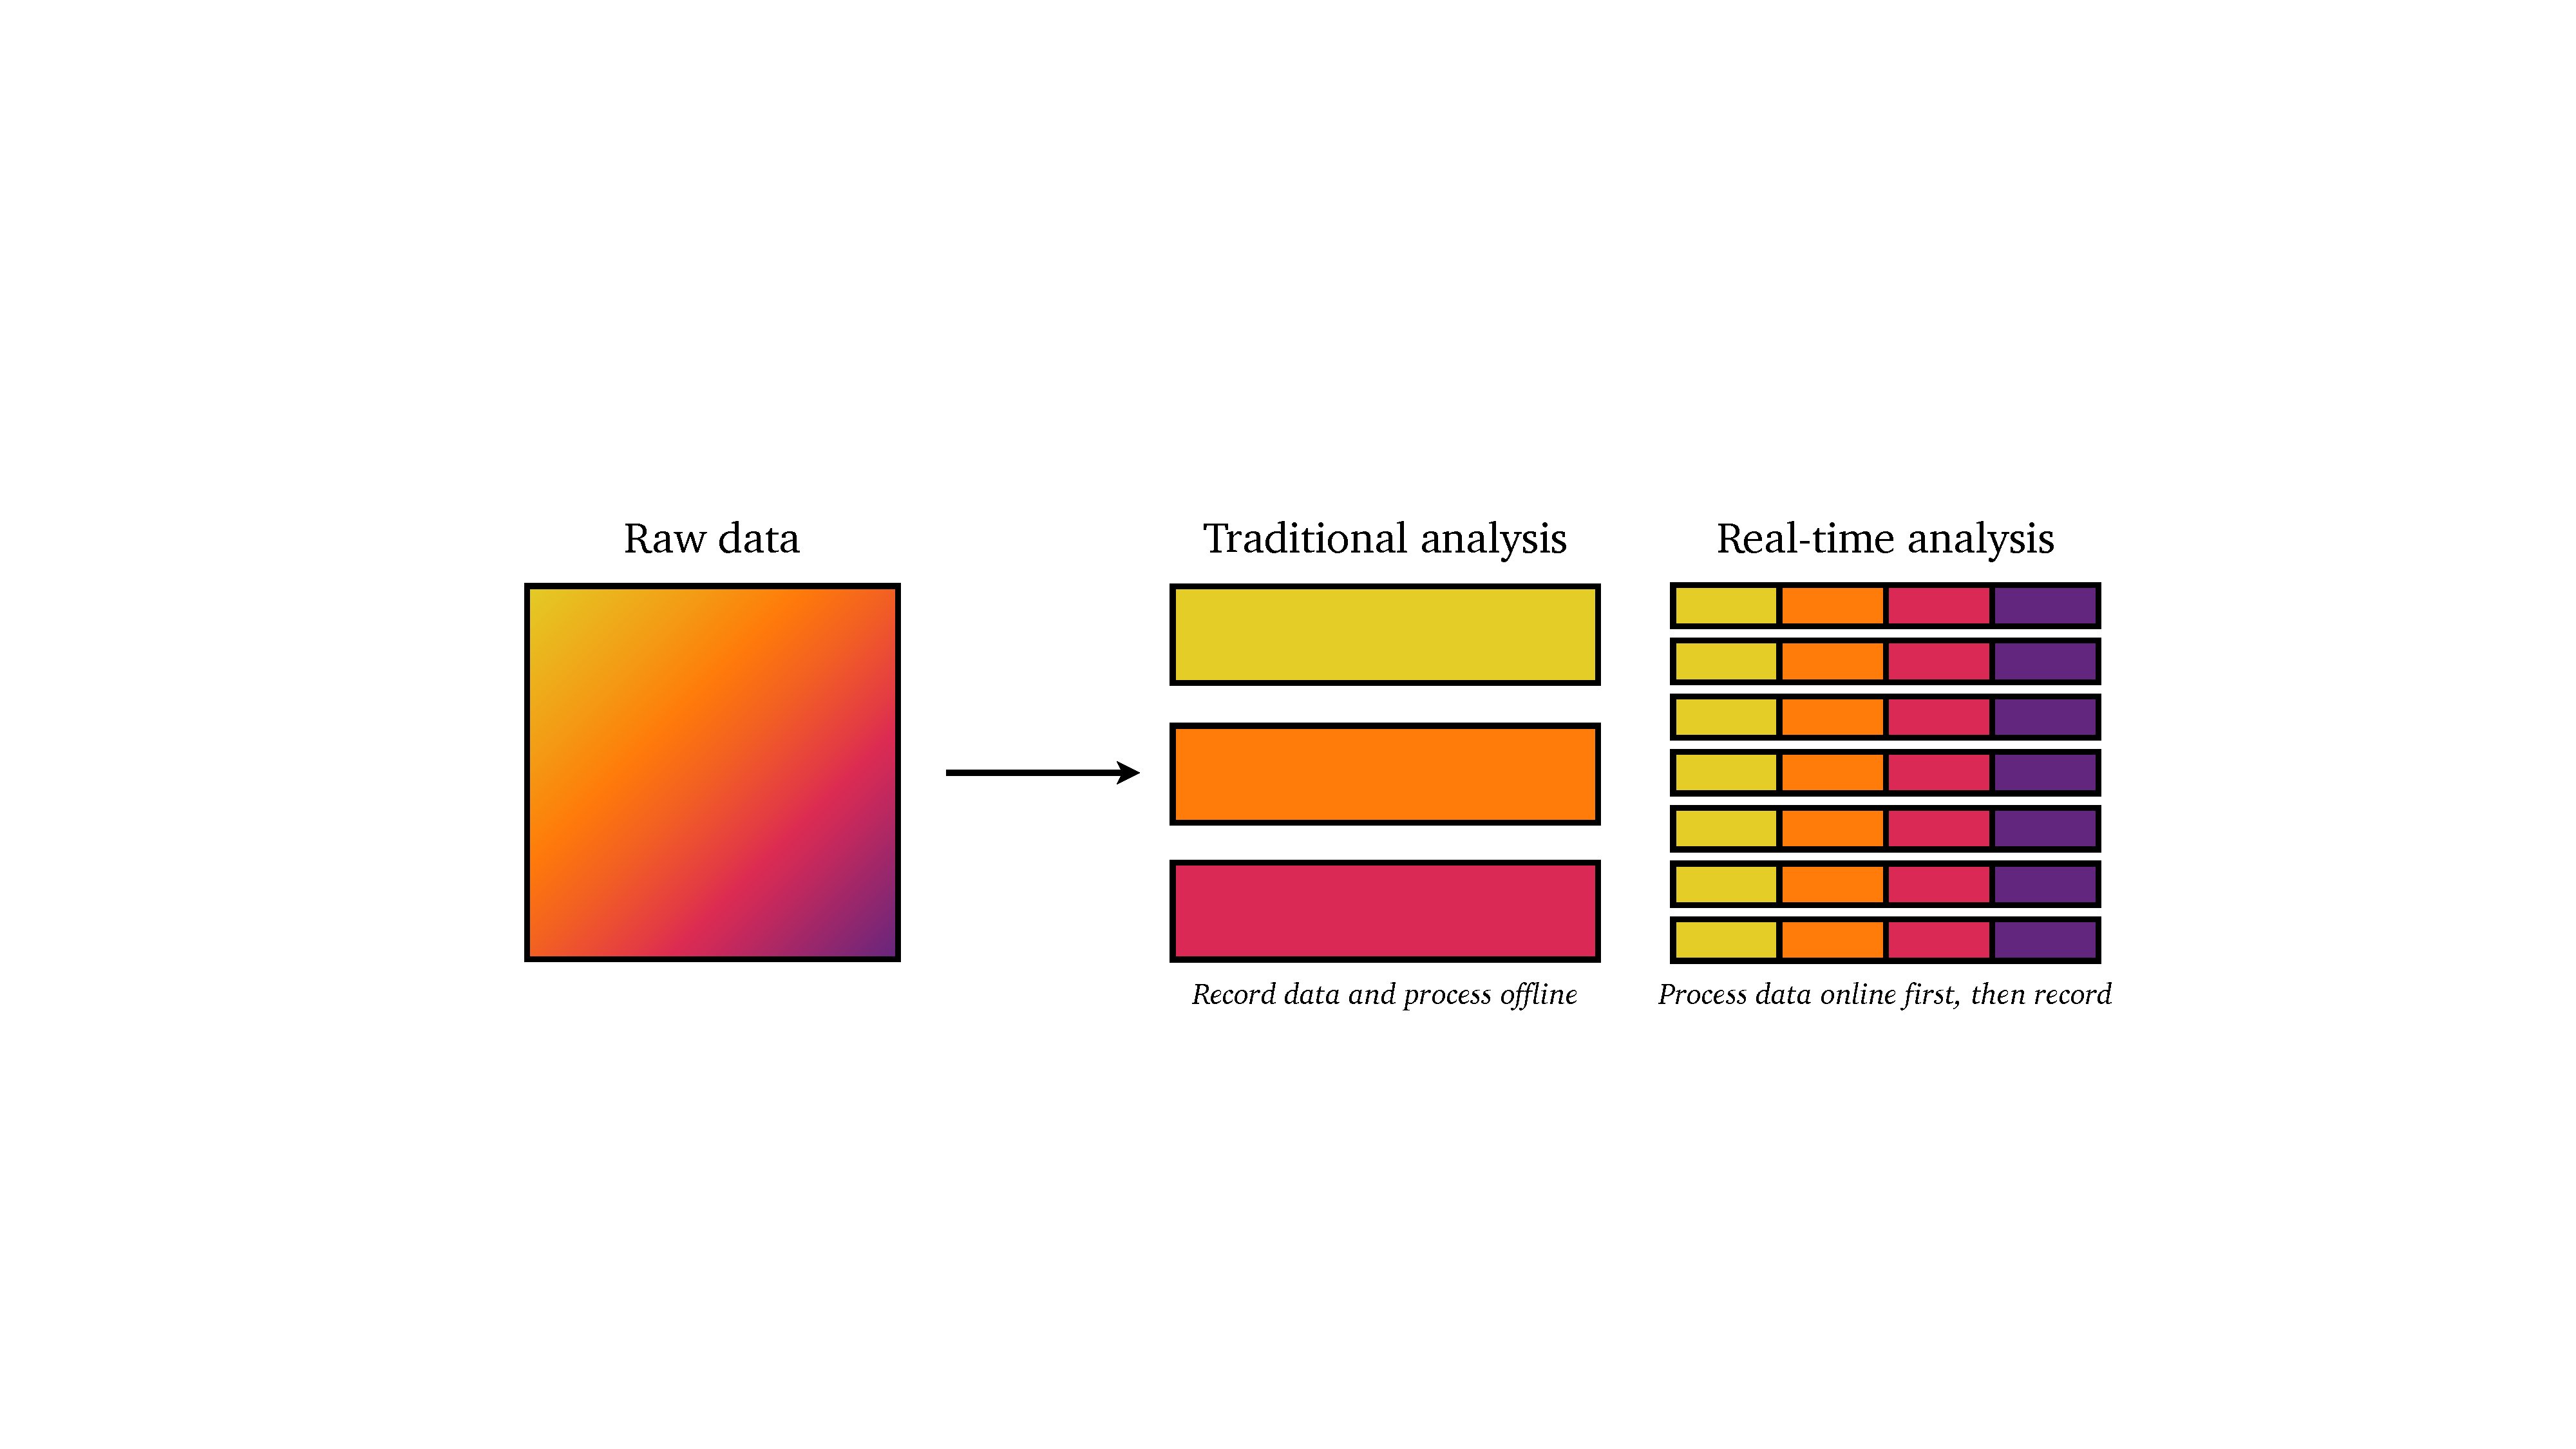
\includegraphics[width=\linewidth]{/Users/jgooding/Documents/SMARTHEP/CHEP2023/CHEP2023/proceedings/figures/rta-diagram.pdf}
    \caption{The traditional and real-time analysis approaches to processing raw data. Traditional approaches rely on recording all data and processing this offilne. Real-time analysis reverses this, processing data as it is produced and recording only the relevant processed information, enabling larger volumes of processed data to be stored.}
    \label{rta-diagram}       % Give a unique label
\end{figure*}
RTA techniques have seen widespread adoption across HEP, in particular amongst trigger and data acquisition (TDAQ) systems. Since it is not possible to record the detector output and carry out event reconstruction at the LHC collision rate of {40}{MHz}, a trigger must be devised to select only those events which are relevant to the physics goals of a given experiment. Such a trigger conventionally consists of a hardware trigger acting directly on parts of the detector output, and a staged software trigger, applying gradually more fine-tuned selections with increasing amounts of reconstructed event detail.\par
In industry, the limitations of the scale of ``big data'' looms over many applications of computing. However, \par
Successful implementation of RTA approaches rests upon the . In particular, in the areas of machine learning and hybrid architectures, which are summarised in Sections~\ref{machine-learning}~\&~\ref{hybrid-architectures}.

\subsection{Machine learning}
\label{machine-learning}
Machine learning (ML), a catch-all for a number of techniques and technologies wherein algorithms are trained to analyse data, enables rapid decision making and pattern recognition across a broad range of use cases. \cite{intro-ml} Whilst general consumer access to ML models is a relatively recent phenomenon, ML already has an extensive history, with the foundations being laid in the 1950s and 1960s. \cite{rosenblatt-ml, neighbours-ml} In HEP, this history begins in the 1990s  with the use of classifiers in offline physics analysis, and has since developed to a variety of classification on pattern recognition/anomaly detection techniques for both online and offline use. \cite{delphi-ml, albertsson-ml}\par

Leading with the firs of these tools, ML classifiers are algorithms classed with classification. Many such algorithms exist, with Boosted Decision Trees (BDTs) and Neural Networks (NNs) amongst those employed across the field. The use of BDTs in signal selection for offline physics analysis has become standard practice, e.g. in suppresion of combinatorial background in the LHCb experiment measurement of the $B_s^0-\bar{B}_s^0$ oscillation frequency. \cite{delta-ms} However, classifiers are also used to aid event reconstruction, e.g. in the CMS boosted event shape tagger, a NN trained to discriminate between possible $t$, $W^\pm$, $Z^0$ and $H$ candidates within an event. \cite{CMS-best} In industry, ML classifiers are used frequently in content deliver\par

Machine learning techniques can also be applied to pattern recognition and anomaly detection—tasks which cannot be realistically carried out on the scales of data presently being analysed. In industry, this is applied intuitively to fraud detection, wherein subtle details in data such as the transactions of a customer. In HEP \cite{anomaly-hep}

\subsection{Hybrid architectures}
\label{hybrid-architectures}
Typical computational resources consist of Central Processing Units (CPUs), processors which are designed for general purpose computation (i.e. varied tasks with significant variety in computing/memory resources), with large on-board memory and often multiple processing cores. Alternative architectures, such as those shown in Figure~\ref{architectures}, can be applied in conjunction or in place of CPU architectures to accelerate processing where tasks are not well-suited are to CPU architectures alones. \par

\begin{figure*}[h!]
    \centering
    % Use the relevant command for your figure-insertion program
    % to insert the figure file. See example above.
    % If not, use
    %\vspace*{5cm}       % Give the correct figure height in cm
    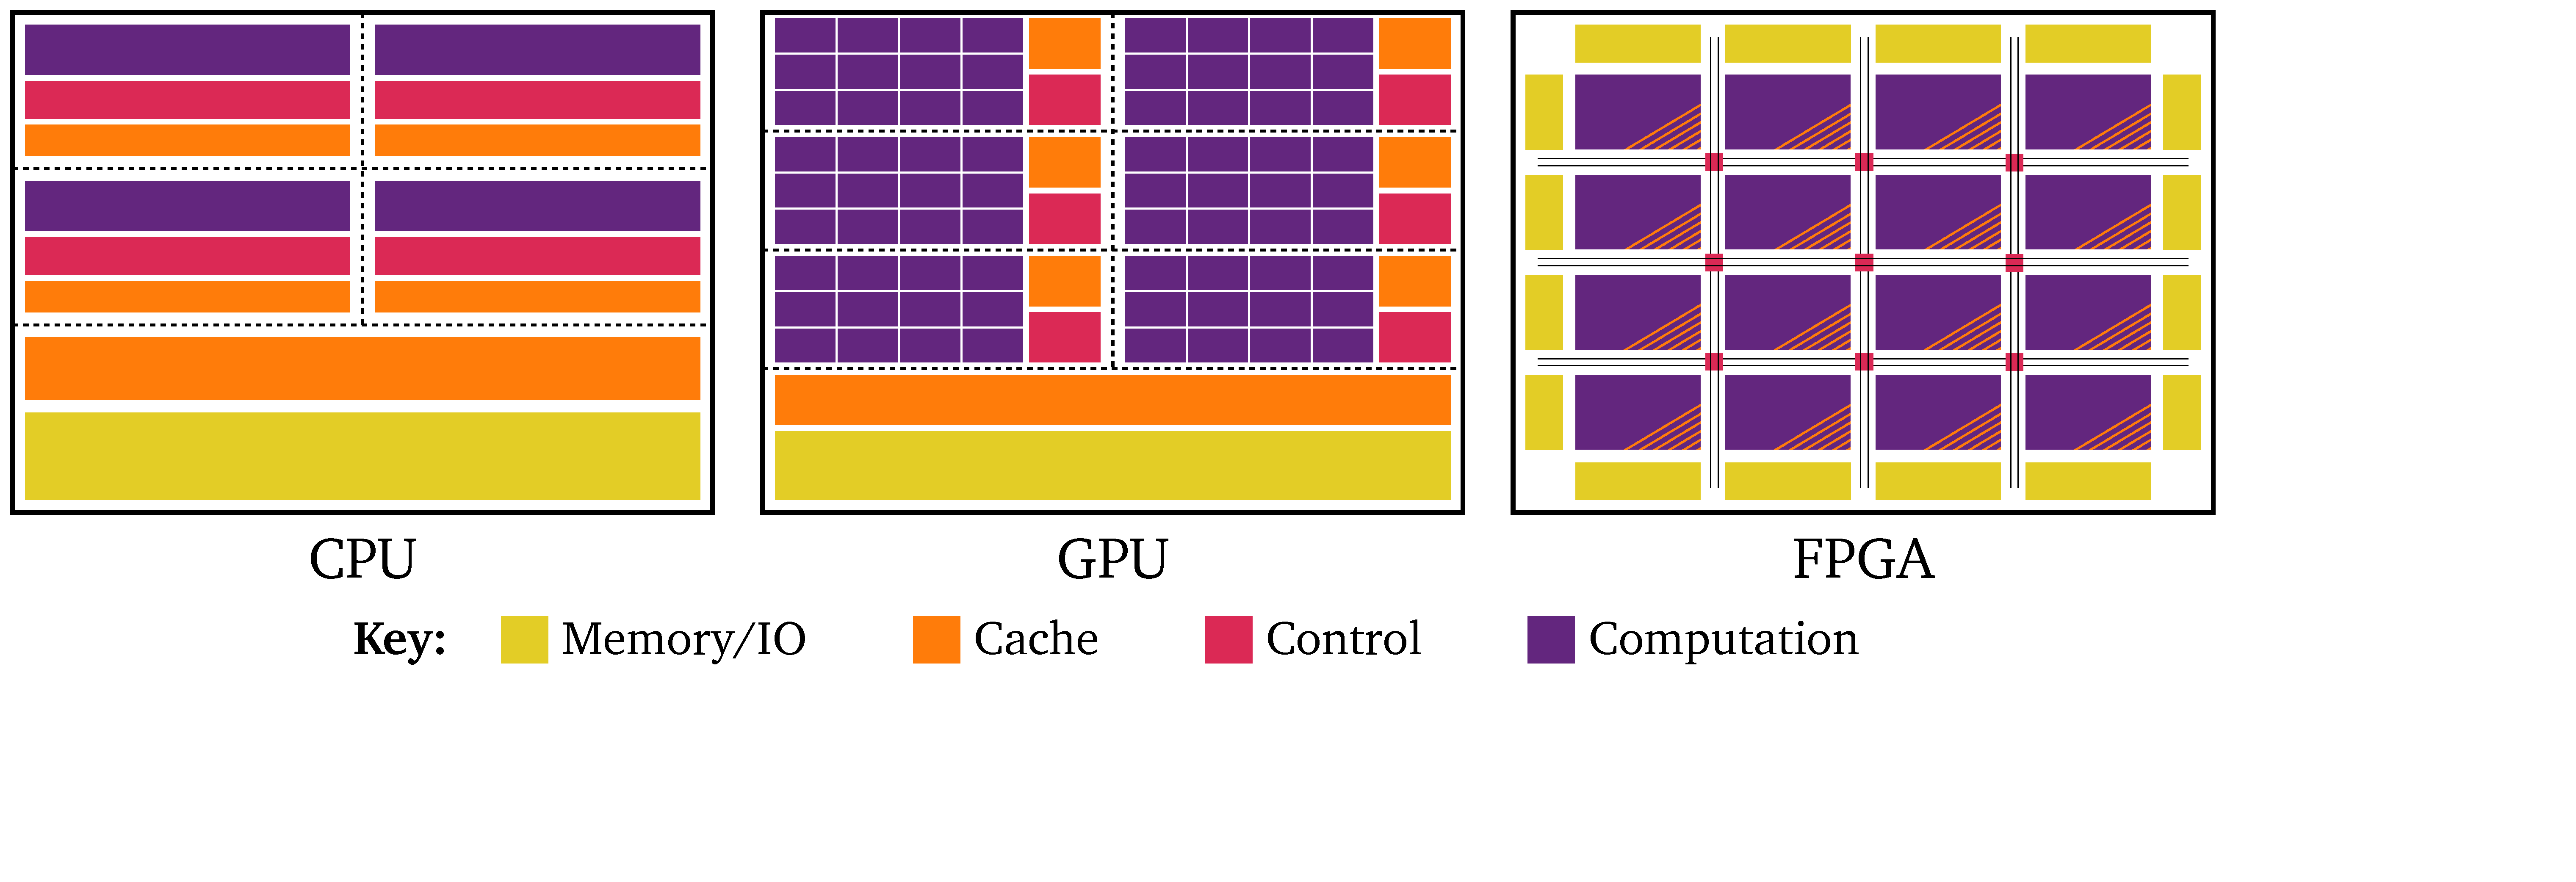
\includegraphics[width=0.9\linewidth,clip]{/Users/jgooding/Documents/SMARTHEP/CHEP2023/CHEP2023/proceedings/figures/architectures-diagram.pdf}
    \caption{Comparison of CPU, GPU and FPGA architectures. A CPU is typically formed of several cores, each containing computational, control and cache resources, and a centralized cache, memory and input/output (IO) interface. GPUs are formed similarly, with centralized cache, memory and IO, and many multiprocessors; however, each multiprocessor contains a greater proportion of computational resources, which are themselves partitioned to perform tasks in parallel. FPGAs are structured in a radically different way, with memory and IO connected to many interlinked control blocks, each primarily formed of simpler logic gate arrangements and often accompanied by a small cache.}
    \label{architectures}       % Give a unique label
\end{figure*}

Field-programmable gate arrays (FPGAs) are integrated circuits which can be programmed by the user for specific tasks. \cite{fpgas-intro} An FPGA consists of many simple logic circuits with a small amount of on-board memory, formed into logic blocks, each of which are connected via switch matrices. \cite{fpgas-book} FPGAs are thus well-suited to bespoke, computationally light but highly parallelisable tasks, such as low-level trigger decisions, wherein simple selections must be made rapidly. \cite{duarte-fpgas} In industry, FPGAs have seen adoption . However; a lack of on-board memory limits the deployment of FPGAs to more intensive tasks.\par
Graphical Processing Units (GPUs) can also be employed to . \cite{vomBruch-gpus} Historically, the use of GPUs has been 
